\documentclass[tikz,border=8pt]{standalone}
\usepackage{tikz}
\usepackage{pgfplots}
\usepackage{amsmath,amssymb}
\usepackage[T1]{fontenc}
\usepackage{lmodern}
\usepackage{xcolor}
\usetikzlibrary{arrows.meta,positioning,shapes.geometric,fit,calc,backgrounds,matrix}
\pgfplotsset{compat=1.18}
\definecolor{ink}{HTML}{18202A}
\definecolor{blue}{HTML}{2563EB}
\definecolor{bluefill}{HTML}{EAF1FF}
\definecolor{green}{HTML}{14804A}
\definecolor{greenfill}{HTML}{E8F6EE}
\definecolor{amber}{HTML}{B56A00}
\definecolor{amberfill}{HTML}{FFF3D6}
\definecolor{red}{HTML}{B42318}
\definecolor{redfill}{HTML}{FDECEC}
\definecolor{gray}{HTML}{667085}
\definecolor{light}{HTML}{F4F6F8}
\definecolor{linegray}{HTML}{C7CDD4}
\tikzset{
  box/.style={draw=ink, rounded corners=3pt, very thick, fill=white, align=center, inner sep=7pt, font=\sffamily\small},
  bluebox/.style={box, fill=bluefill, draw=blue},
  greenbox/.style={box, fill=greenfill, draw=green},
  amberbox/.style={box, fill=amberfill, draw=amber},
  redbox/.style={box, fill=redfill, draw=red},
  ghost/.style={draw=linegray, rounded corners=3pt, thick, fill=light, align=center, inner sep=7pt, font=\sffamily\small},
  label/.style={font=\sffamily\footnotesize, text=gray, align=center},
  title/.style={font=\sffamily\bfseries\large, text=ink, align=center},
  arrow/.style={-{Latex[length=3mm,width=2mm]}, very thick, draw=ink},
  bluearrow/.style={-{Latex[length=3mm,width=2mm]}, very thick, draw=blue},
  redarrow/.style={-{Latex[length=3mm,width=2mm]}, very thick, draw=red},
  greenarrow/.style={-{Latex[length=3mm,width=2mm]}, very thick, draw=green}
}

\begin{document}
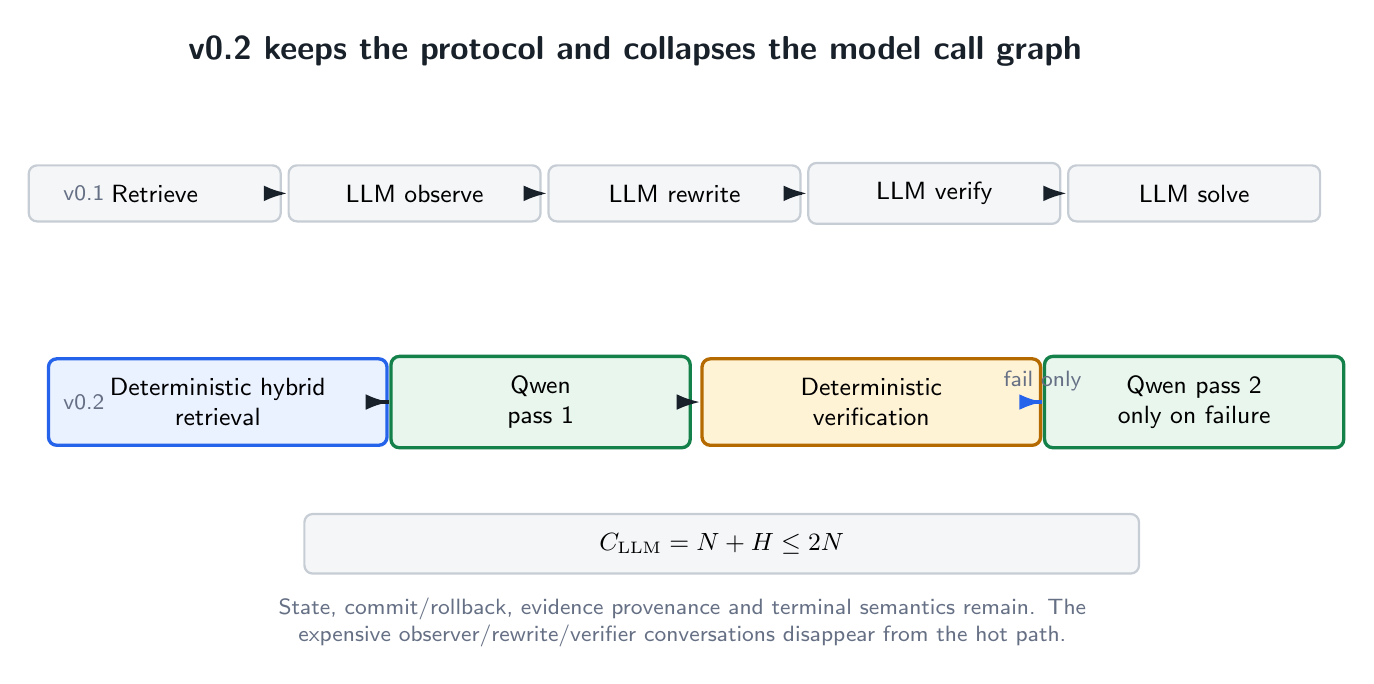
\begin{tikzpicture}
\node[title] at (7.6,5.9) {v0.2 keeps the protocol and collapses the model call graph};
\node[ghost, minimum width=32mm] (a1) at (1.5,4.1) {Retrieve};
\node[ghost, minimum width=32mm] (a2) at (4.8,4.1) {LLM observe};
\node[ghost, minimum width=32mm] (a3) at (8.1,4.1) {LLM rewrite};
\node[ghost, minimum width=32mm] (a4) at (11.4,4.1) {LLM verify};
\node[ghost, minimum width=32mm] (a5) at (14.7,4.1) {LLM solve};
\draw[arrow] (a1)--(a2); \draw[arrow] (a2)--(a3); \draw[arrow] (a3)--(a4); \draw[arrow] (a4)--(a5);
\node[label] at (0.6,4.1) {v0.1};
\node[bluebox, minimum width=43mm] (b1) at (2.3,1.45) {Deterministic hybrid\\retrieval};
\node[greenbox, minimum width=38mm] (b2) at (6.4,1.45) {Qwen\\pass 1};
\node[amberbox, minimum width=43mm] (b3) at (10.6,1.45) {Deterministic\\verification};
\node[greenbox, minimum width=38mm] (b4) at (14.7,1.45) {Qwen pass 2\\only on failure};
\draw[arrow] (b1)--(b2); \draw[arrow] (b2)--(b3); \draw[bluearrow] (b3)--node[label,above]{fail only}(b4);
\node[label] at (0.6,1.45) {v0.2};
\node[ghost, minimum width=106mm] at (8.7,-0.35) {$C_{\mathrm{LLM}}=N+H\le 2N$};
\node[label, text width=145mm] at (8.2,-1.35) {State, commit/rollback, evidence provenance and terminal semantics remain. The expensive observer/rewrite/verifier conversations disappear from the hot path.};
\end{tikzpicture}
\end{document}
